% =====================================================================
% Atividade Prática — Aula 4 — Campo Minado
% Estruturas de Dados — UniLasalle EAD — Prof. Filipo Novo Mór — 2026
% Compilar com XeLaTeX (no Overleaf: Menu > Compiler > XeLaTeX).
% =====================================================================
\documentclass[11pt]{article}
\usepackage{estilo-ed}
\renewcommand{\edcabecalho}{ESTRUTURAS DE DADOS \textbar\ AULA 4 \textbar\ ATIVIDADE PRÁTICA: CAMPO MINADO}
\hypersetup{pdftitle={Atividade Prática - Aula 4 - Campo Minado},
  pdfauthor={Prof. Filipo Novo Mór}, pdfsubject={Estruturas de Dados - UniLasalle EAD}}

% Tabuleiro da Parte A (5 x 5), desenhado em TikZ
\newcommand{\minaTikz}[2]{% coluna, linha (a partir de 1)
  \begin{scope}[shift={(#1-0.5, 5.5-#2)}]
    \foreach \a in {0,45,90,135} \draw[edtexto, line width=1.1pt] (\a:0.3) -- (\a+180:0.3);
    \fill[edtexto] (0,0) circle (0.19);
    \fill[white] (-0.07,0.07) circle (0.045);
  \end{scope}}

\begin{document}
\thispagestyle{primeira}

% ------------------------------- abertura -------------------------------
\begin{minipage}[t]{0.73\textwidth}
  \vspace{0pt}
  {\small\bfseries\color{edteal}ESTRUTURAS DE DADOS · UNILASALLE EAD}\par\vspace{0.7em}
  
\includegraphics[height=0.95cm]{figuras/titulo_atividade.png}\par\vspace{0.25em}
  
\includegraphics[height=1.45cm]{figuras/titulo_campo_minado.png}\par\vspace{0.6em}
  {\large\color{edverde}Integrando Lista, Pilha, Fila e Conjunto — e medindo o custo de cada jogada}\par\vspace{0.5em}
  {\small\color{edcinza}Grau 1 · Aula 4 · Python 3.10+ (ou C11) · Prática de autoestudo, sem entrega · Tempo sugerido: 4 a 6 horas}
\end{minipage}\hfill
\begin{minipage}[t]{0.22\textwidth}
  \vspace{0pt}\raggedleft
  
\includegraphics[width=3.2cm]{figuras/foto_professor.png}
\end{minipage}

\vspace{0.4em}
{\color{edverde}\rule{\textwidth}{1.2pt}}

\begin{objetivo}
Aplicar, em um programa completo, as estruturas das Aulas 1 a 3 — lista contígua, Pilha, Fila
e Conjunto — e analisar o custo de cada parte com as ferramentas da Aula 4: contagem de
operações, notação $O$ e melhor e pior caso.
\end{objetivo}

\begin{semEntrega}
Esta é uma atividade de prática e autoestudo: não há entrega nem nota. Uma solução de exemplo,
completa e comentada, está disponível no repositório da disciplina, junto com o gabarito das
partes sem código. Tente resolver antes de consultá-la: é tentando que se aprende.
\end{semEntrega}

% ------------------------------------------------------------------------
\section{O jogo e as quatro aulas}

O Campo Minado é um jogo de lógica clássico: um tabuleiro de células fechadas esconde algumas
minas, e o jogador precisa abrir todas as células seguras usando as pistas numéricas que
aparecem. Por trás de um jogo simples, há exatamente o que estudamos no Grau 1: uma estrutura
contígua para o tabuleiro, uma Fila (ou uma Pilha) para abrir áreas vazias, um Conjunto para
sortear minas sem repetição, uma Pilha para o histórico de jogadas e, sobre tudo isso, a
pergunta da Aula 4: \emph{quanto custa cada operação?}



\begin{center}
\begin{tabularx}{\textwidth}{>{\centering\arraybackslash}p{1.2cm} P{4.6cm} L}
\cab \tc{Aula} & \tc{Conceito} & \tc{Onde aparece no jogo} \\
1 & Lista contígua, acesso por índice em $O(1)$ & o tabuleiro inteiro é guardado em listas lineares \\
\rowcolor{edfundo} 2 & Fila encadeada (FIFO) & abrir uma área vazia \enquote{em ondas} \\
2 & Pilha contígua (LIFO) & abrir \enquote{em profundidade} e guardar o histórico de jogadas \\
\rowcolor{edfundo} 3 & Conjunto, sem duplicatas & sortear as minas sem repetição e guardar as bandeiras \\
4 & Contagem de operações, $O$, $\Omega$, $\Theta$, casos & contador de operações, ranking com Insertion Sort e a análise da Parte D \\
\end{tabularx}
\end{center}

\begin{figure}[!htb]
  \centering
  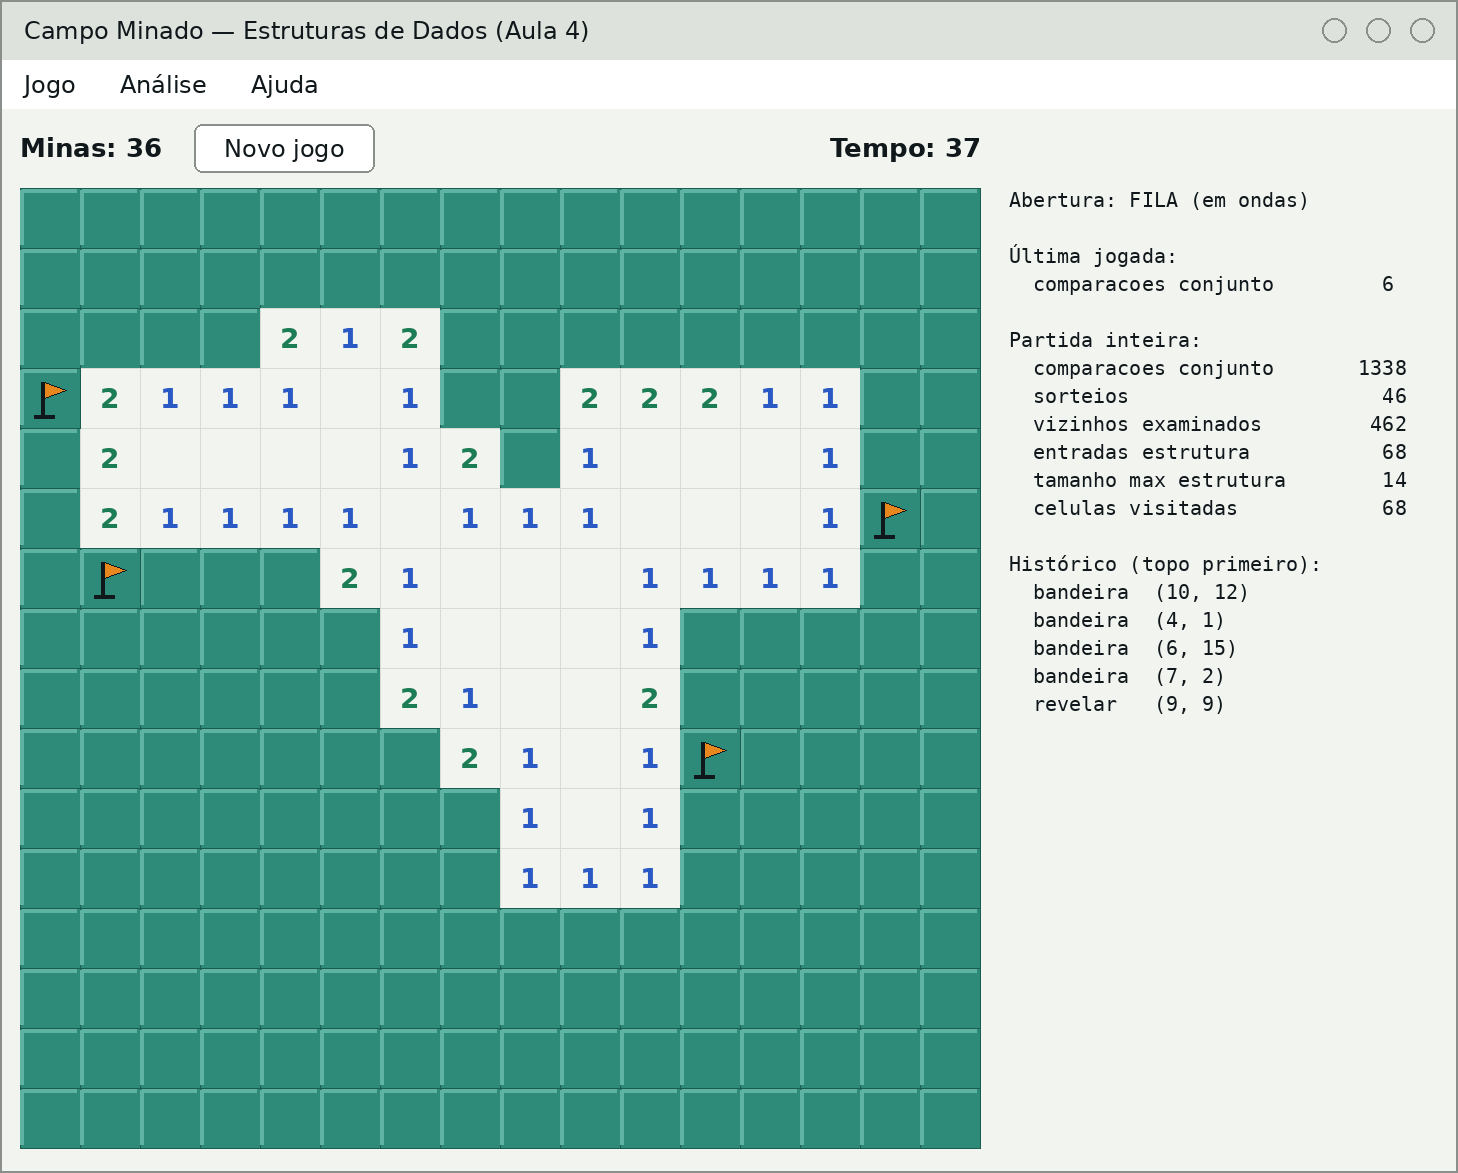
\includegraphics[width=0.84\textwidth]{figuras/janela_campo_minado.png}
  \caption{A interface gráfica do jogo (nível Médio), com o painel de análise à direita.
  Ilustração gerada a partir do código de desenho do próprio jogo.}
\end{figure}

% ------------------------------------------------------------------------
\section{As regras do jogo, em resumo}

\begin{itemize}
  \item O tabuleiro tem $L$ linhas e $C$ colunas de células fechadas; $k$ delas escondem uma mina.
  \item Revelar uma célula com mina encerra a partida com \textbf{derrota}.
  \item Uma célula segura revelada mostra um \textbf{número}: quantas minas existem entre as suas
        até 8 vizinhas (em cima, embaixo, dos lados e nas diagonais).
  \item Uma célula com \textbf{0} não tem minas em volta; por isso o jogo abre automaticamente as
        suas vizinhas — e as vizinhas das vizinhas que também forem 0. É a \textbf{abertura em cascata}.
  \item O jogador pode marcar uma \textbf{bandeira} onde acha que há uma mina. Células com
        bandeira não podem ser reveladas (nem pela cascata) até a bandeira ser retirada.
  \item O \textbf{primeiro clique é sempre seguro}: as minas só são sorteadas depois dele, longe
        da célula clicada e das suas vizinhas.
  \item A partida termina com \textbf{vitória} quando todas as células seguras estão abertas.
\end{itemize}

\begin{center}
\begin{tabularx}{0.72\textwidth}{L C C}
\cab \tc{Nível} & \tc{Tabuleiro} & \tc{Minas} \\
Fácil & $9 \times 9$ & 10 \\
\rowcolor{edfundo} Médio & $16 \times 16$ & 40 \\
Difícil & $16 \times 30$ & 99 \\
\end{tabularx}
\end{center}

\begin{naapostila}
O capítulo 14 da apostila da Aula 4, \enquote{Campo Minado: regras do jogo e técnicas de
implementação}, traz as regras em detalhes, com exemplos passo a passo, e explica cada
algoritmo e técnica usados nesta atividade.
\end{naapostila}

% ------------------------------------------------------------------------
\section{Arquivos e regras}

Os arquivos estão na pasta \codigo{aula04-complexidade} do repositório da disciplina,
\url{https://github.com/ProfessorFilipo/EstruturasDados}:

\begin{arvore}
aula04-complexidade/
├── exercicios/campo_minado/     <- ESQUELETO: comece por aqui
│   ├── tabuleiro.py             <- TODOs 1 a 10 (a lógica do jogo)
│   ├── ranking.py               <- TODOs 11 e 12
│   ├── estruturas.py            <- Pilha, Fila e Conjunto (prontos)
│   ├── jogo_gui.py              <- interface gráfica (pronta)
│   ├── jogo_terminal.py         <- interface de texto (pronta)
│   ├── testes.py                <- testes automáticos (prontos)
│   ├── analise_complexidade.py  <- medições da Parte D (pronto)
│   └── campo_minado_arquivo_unico.py   <- tudo em um arquivo, para IDE online
└── solucoes/campo_minado/       <- SOLUÇÃO DE EXEMPLO e GABARITO.md
\end{arvore}

\begin{itemize}
  \item Complete somente os trechos marcados com \codigo{TODO}. Não mude nomes nem parâmetros
        dos métodos: as interfaces e os testes dependem deles.
  \item Em \codigo{tabuleiro.py}, não use \codigo{set()}, \codigo{collections.deque} nem
        \codigo{queue.Queue}: use a \codigo{Pilha}, a \codigo{Fila} e o \codigo{Conjunto} de
        \codigo{estruturas.py} — as mesmas das Aulas 2 e 3.
  \item Use só a biblioteca padrão do Python (nada de \codigo{pip install}).
  \item No código, linhas e colunas começam em 0. As interfaces mostram a partir de 1 para o
        jogador: a célula que ele chama de (5,\,1) é a (4,\,0) no código.
\end{itemize}

% ------------------------------------------------------------------------
\section{Preparando o ambiente}

\subsection{Python e PyCharm, passo a passo (Windows)}

\begin{enumerate}
  \item \textbf{Instale o Python.} Em \href{https://www.python.org/downloads/}{python.org/downloads},
        baixe a versão mais recente do Python 3. Na primeira tela do instalador, marque a opção
        \textbf{Add python.exe to PATH} e clique em \textbf{Install Now}. A instalação padrão já
        inclui o tkinter, usado pela interface gráfica.
  \item \textbf{Confira a instalação.} Abra o Prompt de Comando e digite \codigo{py --version}.
        Deve aparecer algo como \codigo{Python 3.12.x}.
  \item \textbf{Instale o PyCharm.} Em \href{https://www.jetbrains.com/pycharm/download/}{jetbrains.com/pycharm/download},
        baixe e instale o PyCharm. As funções essenciais são gratuitas e bastam para esta atividade.
  \item \textbf{Baixe os arquivos.} Na página do repositório no GitHub, clique no botão verde
        \textbf{Code} e depois em \textbf{Download ZIP}. Descompacte o arquivo em uma pasta sua.
  \item \textbf{Abra a pasta do esqueleto.} No PyCharm, use \textbf{File > Open} e escolha a pasta
        \codigo{aula04-complexidade/exercicios/campo_minado}.
  \item \textbf{Confira o interpretador.} No canto inferior direito da janela, o PyCharm mostra a
        versão do Python em uso. Se aparecer \enquote{No interpreter}, clique ali e escolha o Python
        que você instalou.
  \item \textbf{Rode o jogo.} Clique com o botão direito em \codigo{jogo_gui.py} e escolha
        \textbf{Run}. A janela abre; ao clicar numa célula, aparece o aviso
        \enquote{Falta implementar: TODO 1}. É por aí que você começa.
  \item \textbf{Rode os testes.} Da mesma forma, rode \codigo{testes.py}. Faça isso depois de
        cada TODO para conferir o que já está certo.
\end{enumerate}

\subsection{Outras opções}

\begin{itemize}
  \item \textbf{Thonny} (\href{https://thonny.org}{thonny.org}): um editor gratuito e bem simples,
        que já vem com o Python e o tkinter. Boa opção para computadores mais modestos: abra o
        arquivo e tecle \textbf{F5} para rodar.
  \item \textbf{Só IDE online:} use \codigo{campo_minado_arquivo_unico.py} no
        \href{https://www.onlineide.pro/playground/python}{onlineide.pro/playground/python}. É a
        versão de texto, com todo o código em um único arquivo. A interface gráfica não funciona
        em IDEs online.
  \item \textbf{macOS:} o Python do python.org já traz o tkinter; use \codigo{python3} no Terminal.
        O clique direito do jogo também funciona com \textbf{Control + clique}.
  \item \textbf{Linux:} se aparecer \codigo{No module named 'tkinter'}, instale o pacote do
        sistema (no Ubuntu/Debian: \codigo{sudo apt install python3-tk}).
  \item \textbf{Linguagem C:} o CLion (gratuito para uso não comercial, como estudo) ou o
        Code::Blocks (escolha o instalador que já inclui o compilador MinGW). Veja a seção 10.
\end{itemize}

% ------------------------------------------------------------------------
\section{Parte A — Modelagem no papel, antes do código}

Resolva esta parte com lápis e papel. Ela é a base de tudo o que você vai programar depois,
e o \codigo{testes.py} usa exatamente este tabuleiro.

\begin{figure}[H]
\centering
\begin{tikzpicture}[scale=0.82]
  % tabuleiro 5x5 com as minas
  \fill[edfundo] (0,0) rectangle (5,5);
  \draw[edcinzaclaro, line width=0.8pt] (0,0) grid (5,5);
  \draw[edverde, line width=1.2pt] (0,0) rectangle (5,5);
  \foreach \i in {1,...,5} {
    \node[font=\small\bfseries, color=edverde] at (\i-0.5, 5.35) {\i};
    \node[font=\small\bfseries, color=edverde] at (-0.35, 5.5-\i) {\i};
  }
  \node[font=\footnotesize, color=edcinza] at (2.5, 6.0) {coluna};
  \node[font=\footnotesize, color=edcinza, rotate=90] at (-0.95, 2.5) {linha};
  \minaTikz{4}{1} \minaTikz{2}{2} \minaTikz{5}{4}
  \draw[edlaranja, line width=2pt] (0.06,0.06) rectangle (0.94,0.94);
  \node[font=\footnotesize\bfseries, color=edlaranja, anchor=north] at (0.5,-0.1) {clique};
  % ordem das vizinhas
  \begin{scope}[shift={(8,1)}]
    \fill[edfundo] (0,0) rectangle (3,3);
    \draw[edcinzaclaro, line width=0.8pt] (0,0) grid (3,3);
    \draw[edverde, line width=1.2pt] (0,0) rectangle (3,3);
    \fill[edteal] (1.08,1.08) rectangle (1.92,1.92);
    \node[font=\bfseries, color=white] at (1.5,1.5) {X};
    \foreach \n/\x/\y in {1/0.5/2.5, 2/1.5/2.5, 3/2.5/2.5, 4/0.5/1.5, 5/2.5/1.5, 6/0.5/0.5, 7/1.5/0.5, 8/2.5/0.5}
      \node[font=\large\bfseries, color=edverde] at (\x,\y) {\n};
    \node[font=\footnotesize, color=edcinza, align=center] at (1.5,-0.55) {ordem de exame\\das vizinhas de X};
  \end{scope}
\end{tikzpicture}
\caption{À esquerda, o tabuleiro da Parte A: 5 × 5, com minas em (1,\,4), (2,\,2) e (4,\,5), e o
clique em (5,\,1). À direita, a ordem em que as vizinhas devem ser examinadas:
noroeste, norte, nordeste, oeste, leste, sudoeste, sul e sudeste.}
\end{figure}

\begin{enumerate}[label={\color{edverde}\bfseries A\arabic*.}, leftmargin=2.2em]
  \item \textbf{Números.} Desenhe o tabuleiro e escreva, em cada célula segura, quantas minas há
        entre as suas vizinhas. Atenção às bordas e aos cantos: uma célula de canto tem só 3
        vizinhas; uma de borda, 5.
  \item \textbf{Índices.} O tabuleiro será guardado em uma lista linear de 25 posições. Contando
        linhas e colunas a partir de 1, a célula (linha, coluna) fica na posição
        $\text{índice} = (\text{linha} - 1) \times 5 + (\text{coluna} - 1)$.
        Calcule o índice de (1,\,4), (2,\,2) e (4,\,5). Depois faça o caminho inverso: qual célula
        está no índice 12?
  \item \textbf{Abertura com Fila.} Simule o clique em (5,\,1) usando uma Fila. Comece colocando
        (5,\,1) na fila e, a cada passo, retire a célula da frente; se o número dela for 0,
        coloque na fila as vizinhas ainda fechadas, na ordem da figura. Registre cada passo:
\end{enumerate}

\begin{center}
\begin{tabularx}{\textwidth}{>{\centering\arraybackslash}p{1.1cm} >{\centering\arraybackslash}p{1.9cm} >{\centering\arraybackslash}p{1.4cm} >{\centering\arraybackslash}p{3.4cm} L}
\cab \tc{Passo} & \tc{Sai da fila} & \tc{Número} & \tc{Entram na fila} & \tc{Fila depois do passo} \\
0 & — & — & (5,1) & (5,1) \\
\rowcolor{edfundo} 1 & (5,1) & 0 & (4,1) (4,2) (5,2) & (4,1) (4,2) (5,2) \\
2 & \dots & & & \\
\rowcolor{edfundo} \dots & & & & \\
\end{tabularx}
\end{center}

\begin{enumerate}[label={\color{edverde}\bfseries A\arabic*.}, leftmargin=2.2em, start=4]
  \item \textbf{Abertura com Pilha.} Repita a simulação trocando a Fila por uma Pilha (a célula
        que sai é sempre a do topo). As células abertas são as mesmas? E a ordem?
  \item \textbf{Placar.} Quantas células foram abertas pelo clique? Quantas células seguras ainda
        faltam abrir para vencer?
\end{enumerate}

\begin{atencao}
Marque cada célula como aberta \textbf{no momento em que ela entra} na estrutura, e não quando
ela sai. Assim nenhuma célula entra duas vezes — e você vai medir, na Parte D, quanto trabalho
isso economiza.
\end{atencao}

\begin{checkpoint}
O clique abre 12 células — as mesmas com Fila e com Pilha — e restam 10 células seguras
fechadas. Com a Fila, as primeiras a sair são (5,\,1), (4,\,1), (4,\,2) e (5,\,2). As tabelas
completas estão no \codigo{GABARITO.md}, na pasta da solução.
\end{checkpoint}

% ------------------------------------------------------------------------
\section{Parte B — O núcleo do jogo (TODOs 1 a 7)}

Todos estes TODOs ficam em \codigo{tabuleiro.py}. Leia o comentário de cada método: ele diz o
que fazer, quais contadores atualizar e qual é o custo esperado.

\begin{center}
\begin{tabularx}{\textwidth}{>{\centering\arraybackslash}p{1.1cm} P{4.4cm} L >{\centering\arraybackslash}p{1.9cm}}
\cab \tc{TODO} & \tc{Método} & \tc{O que faz} & \tc{Custo} \\
1 & \codigo{indice()} & (linha, coluna) $\to$ posição na lista & $O(1)$ \\
\rowcolor{edfundo} 2 & \codigo{coordenadas()} & posição na lista $\to$ (linha, coluna) & $O(1)$ \\
3 & \codigo{vizinhos()} & as até 8 vizinhas, dentro do tabuleiro & $O(1)$ \\
\rowcolor{edfundo} 4 & \codigo{_posicionar_minas()} & sorteio sem repetição, protegendo o 1º clique & $O(k^2)$ \\
5 & \codigo{_calcular_numeros()} & quantas minas há em volta de cada célula & $O(k)$ \\
\rowcolor{edfundo} 6 & \codigo{_abrir_a_partir_de()} & abertura em cascata com Fila ou Pilha & $O(L \cdot C)$ \\
7 & \codigo{_revelar()} & regras da jogada: derrota, abertura, vitória & — \\
\end{tabularx}
\end{center}

\subsubsection{TODOs 1 e 2 — endereçamento [Aula 1]}
Com colunas contadas a partir de 0: \codigo{indice = linha * colunas + coluna}. Para voltar, use a
divisão inteira e o resto: \codigo{linha = indice // colunas} e \lstinline[style=inline]|coluna = indice % colunas|.
Com 5 colunas, (1,\,0) $\to$ 5 e 12 $\to$ (2,\,2).

\subsubsection{TODO 3 — vizinhas}
Percorra a tupla \codigo{DIRECOES}, que já está no arquivo, na ordem em que ela aparece (os testes
conferem a ordem). Para cada deslocamento, calcule a linha e a coluna vizinhas e guarde o índice
só se \codigo{0 <= l < linhas} e \codigo{0 <= c < colunas}. Sem essa verificação, a célula da
última coluna \enquote{enxergaria} a primeira coluna da linha de baixo.

\subsubsection{TODO 4 — sorteio das minas [Aula 3]}
Monte um \codigo{Conjunto} com as células proibidas (a clicada e suas vizinhas). Depois, enquanto
o Conjunto de minas tiver menos que \codigo{num_minas} elementos, sorteie um índice com
\codigo{self._gerador.randrange(self.total_celulas)}, conte em \codigo{"sorteios"} e insira-o se
não for proibido — o Conjunto já ignora repetições. No fim, faça
\codigo{self.minas_posicionadas = True} e chame \codigo{self._calcular_numeros()}.

\subsubsection{TODO 5 — números [Aula 4]}
Não pergunte a cada célula \enquote{quantas vizinhas são minas?}: isso custaria $O(L \cdot C \cdot k)$.
Faça o contrário: percorra só as minas (\codigo{self.minas.valores()}) e some 1 no número de cada
vizinha. São no máximo 8 passos por mina, ou seja, $O(k)$.

\subsubsection{TODO 6 — abertura em cascata [Aula 2]}
Em Python, funções também são valores: guarde em variáveis as operações de colocar e retirar da
estrutura escolhida, e o resto do algoritmo fica igual para Fila e Pilha.

\needspace{6\baselineskip}
\begin{lstlisting}
usar_fila = self.estrategia == "fila"
pendentes = Fila() if usar_fila else Pilha(self.total_celulas)
colocar = pendentes.enfileirar if usar_fila else pendentes.empilhar
retirar = pendentes.desenfileirar if usar_fila else pendentes.desempilhar
\end{lstlisting}

A ideia do algoritmo, em português:

\needspace{8\baselineskip}
\begin{lstlisting}[style=terminal]
marque 'inicio' como revelada e coloque na estrutura
enquanto a estrutura não estiver vazia:
    retire uma célula e acrescente-a à lista 'ordem'
    se o número dela for 0:
        para cada vizinha ainda fechada e sem bandeira:
            marque como revelada e coloque na estrutura
devolva 'ordem'
\end{lstlisting}

Não esqueça os contadores descritos no comentário do método. O teste
\codigo{test_cada_celula_entra_uma_unica_vez} confere que, num tabuleiro $12 \times 12$ sem
minas, exatamente 144 células entram na estrutura.

\subsubsection{TODO 7 — a jogada \enquote{revelar}}
Siga as regras na ordem do comentário: ignore células abertas ou com bandeira; sorteie as minas
se for a primeira jogada; registre \codigo{("revelar", linha, coluna)} no histórico; se for mina,
derrota; senão, abra em cascata e, se \codigo{celulas_seguras_restantes} chegar a 0, vitória.

% ------------------------------------------------------------------------
\section{Parte C — Bandeiras, histórico e ranking (TODOs 8 a 12)}

\begin{itemize}
  \item \textbf{TODO 8 — \codigo{_alternar_bandeira()}:} marca a bandeira ou a retira, se já
        existir (Conjunto: \codigo{pertence}, \codigo{inserir}, \codigo{remover}). Não vale em
        célula aberta. Registre \codigo{("bandeira", linha, coluna)} no histórico.
  \item \textbf{TODO 9 — \codigo{_desfazer()}:} consulte o \textbf{topo} da Pilha. Se for uma
        bandeira, desempilhe e desfaça; se for um \enquote{revelar}, não faça nada — abrir uma
        célula não tem volta. É o comportamento LIFO: só o topo é acessível.
  \item \textbf{TODO 10 — \codigo{ultimas_jogadas()}:} devolva as jogadas mais recentes, do topo
        para a base, \textbf{sem} remover nada da Pilha.
  \item \textbf{TODO 11 — \codigo{inserir_ordenado()}}, em \codigo{ranking.py}: coloque o novo
        recorde no fim da lista e desloque para a direita os anteriores com tempo
        \textbf{maior} — exatamente o laço interno do Insertion Sort. Em caso de empate, o
        recorde mais antigo fica na frente.
  \item \textbf{TODO 12 — \codigo{ordenar_por_insercao()}:} o Insertion Sort completo, usado ao
        carregar o arquivo do ranking. Como o próprio jogo salva o arquivo já ordenado, esse é o
        \textbf{melhor caso} do algoritmo, visto em aula.
\end{itemize}

% ------------------------------------------------------------------------
\section{Parte D — Análise de complexidade}

Quando todos os testes passarem, rode \codigo{analise_complexidade.py} e use a saída para
responder. Use $L$ para linhas, $C$ para colunas, $k$ para minas e $f$ para bandeiras.

\begin{enumerate}[label={\color{edverde}\bfseries D\arabic*.}, leftmargin=2.3em, itemsep=0.45em]
  \item Qual é o custo de \codigo{indice()} e de \codigo{coordenadas()}? Por quê?
  \item Qual é o custo de \codigo{vizinhos()}? Ele depende do tamanho do tabuleiro?
  \item Compare as duas formas de calcular os números, preenchendo a tabela abaixo com a saída do
        programa. Qual é o custo de cada uma, em notação $O$? Quantas vezes a forma ingênua é mais
        cara no nível Difícil?
  \item O sorteio das minas insere cada mina em um Conjunto implementado sobre uma lista. Mostre
        que o total de comparações cresce como $k^2/2$ (dica: soma de Gauss). Que alternativa
        evitaria as repetições do sorteio, e quando ela valeria mais a pena?
  \item Por que a célula é marcada ao \textbf{entrar} na estrutura, e não ao sair? Compare as duas
        colunas da seção 2 da análise.
  \item Fila e Pilha abrem as mesmas células? Na mesma ordem? Com o mesmo custo de tempo? E de
        memória — compare os tamanhos máximos da seção 1 da análise.
  \item Qual é o custo de verificar a vitória com o contador \codigo{celulas_seguras_restantes}?
        E se, a cada jogada, varrêssemos a lista \codigo{reveladas}?
  \item As bandeiras ficam em um Conjunto. Qual é o custo de \codigo{pertence()} nele, e como isso
        afeta a abertura em cascata no pior caso? Como deixar essa consulta em $O(1)$, e qual é o
        preço dessa troca?
  \item Qual é o melhor e o pior caso de \codigo{inserir_ordenado()}? Em que caso do Insertion Sort
        cai o \codigo{ordenar_por_insercao()} ao carregar o arquivo salvo pelo próprio jogo?
  \item Resuma o custo de uma partida: o primeiro clique, cada clique seguinte, cada bandeira e
        cada redesenho do tabuleiro.
\end{enumerate}

\begin{center}
\begin{tabularx}{0.9\textwidth}{L C C C C}
\cab \tc{Nível} & \tcx{$L \times C$} & \tcx{$k$} & \tc{Percorrendo minas} & \tc{Perguntando a cada célula} \\
Fácil & 9 × 9 & 10 & & \\
\rowcolor{edfundo} Médio & 16 × 16 & 40 & & \\
Difícil & 16 × 30 & 99 & & \\
\end{tabularx}
\end{center}

% ------------------------------------------------------------------------
\section{Parte E — Interface gráfica e desafios opcionais}

A interface gráfica (\codigo{jogo_gui.py}) já vem pronta e usa a sua classe \codigo{Tabuleiro}.
Clique esquerdo revela; clique direito (ou Control + clique, no Mac) marca bandeira;
\textbf{Ctrl+Z} desfaz a última bandeira; \textbf{F2} começa um novo jogo. Experimente:

\begin{itemize}
  \item No menu \textbf{Análise}, escolha \textbf{Abrir com Pilha} e ative \textbf{Numerar a ordem
        de abertura}. Clique numa área vazia e compare com a Fila.
  \item Observe o \textbf{painel de análise}: o primeiro clique custa muito mais que os outros. Por quê?
  \item Marque uma bandeira e tecle Ctrl+Z. Depois revele uma célula e tente de novo.
\end{itemize}

\begin{figure}[!htb]
  \centering
  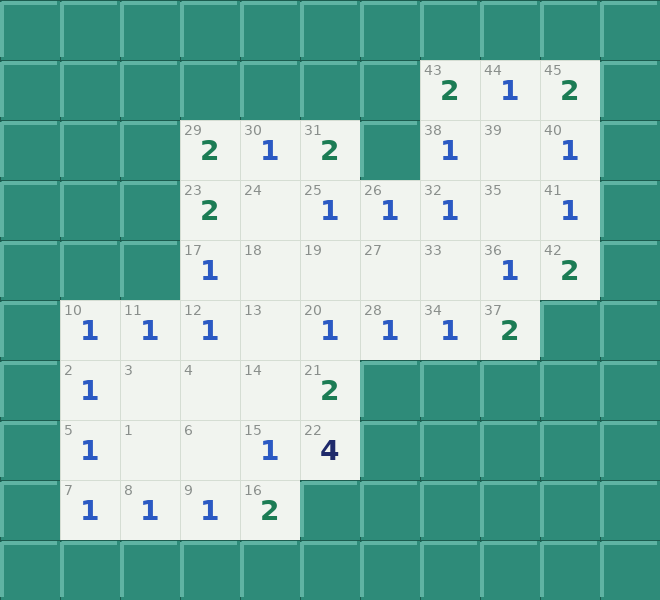
\includegraphics[width=0.46\textwidth]{figuras/ordem_fila.png}\hfill
  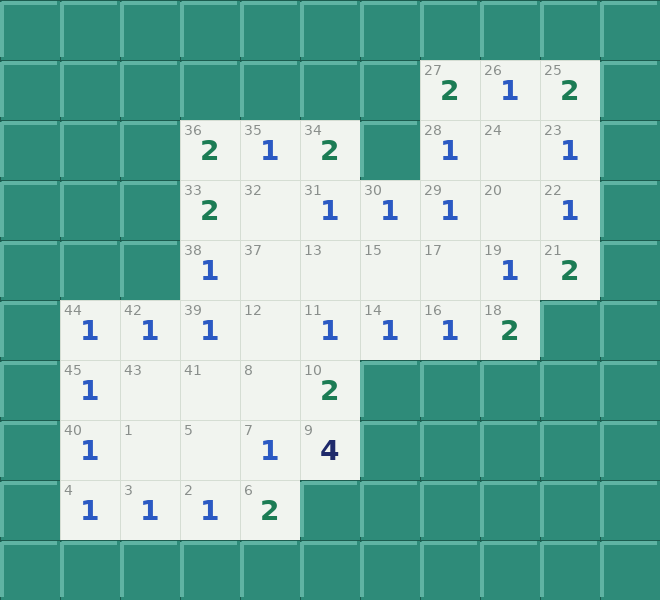
\includegraphics[width=0.46\textwidth]{figuras/ordem_pilha.png}
  \caption{Mesmo tabuleiro, mesmo clique: à esquerda com Fila, à direita com Pilha. Os números
  pequenos mostram a ordem em que as células foram abertas.}
\end{figure}

\textbf{Desafios opcionais}, para quem quiser ir além:
\begin{itemize}
  \item \textbf{Abertura por acorde:} clicar num número já aberto abre as vizinhas, se a
        quantidade de bandeiras em volta for igual ao número.
  \item \textbf{Bandeiras em $O(1)$:} troque o Conjunto de bandeiras por uma lista de booleanos e
        meça a diferença com o \codigo{analise_complexidade.py}.
  \item \textbf{Sorteio por embaralhamento (Fisher–Yates):} implemente e compare o número de
        comparações com o sorteio atual, principalmente com muitas minas.
  \item \textbf{Nível personalizado} na interface gráfica.
\end{itemize}

% ------------------------------------------------------------------------
\section{Para quem escolher a linguagem C}

Em C, faça a versão de terminal, com as mesmas Partes A a D, e use a solução em Python como
referência da lógica. Reaproveite as estruturas das aulas anteriores: a Pilha de
\codigo{aula02-pilhas-filas/c/pilha.c}, a Fila encadeada de \codigo{fila.c} (lembre-se do
\codigo{free} ao desenfileirar) e o Conjunto de \codigo{aula03-conjuntos/c/demo_conjunto.c},
aumentando a capacidade para caber o tabuleiro. Uma organização possível:

\needspace{14\baselineskip}
\begin{lstlisting}[style=c]
#define MAX_CELULAS (16 * 30)          /* maior tabuleiro: nível Difícil */

typedef struct {
    int linhas, colunas, num_minas, total;
    int numeros[MAX_CELULAS];          /* [Aula 1] lista contígua        */
    int reveladas[MAX_CELULAS];        /* 1 = aberta, 0 = fechada        */
    Conjunto minas;                    /* [Aula 3]                       */
    Conjunto bandeiras;                /* [Aula 3]                       */
    Pilha historico;                   /* [Aula 2] jogadas codificadas   */
    int estado;                        /* JOGANDO, VITORIA ou DERROTA    */
    int seguras_restantes;             /* vitória em O(1)                */
} Tabuleiro;
\end{lstlisting}

\begin{itemize}
  \item Uma jogada cabe em um único \codigo{int}: \codigo{jogada = indice * 2 + e_bandeira}.
        Para decodificar: \codigo{indice = jogada / 2} e \lstinline[style=inline]|e_bandeira = jogada % 2|.
  \item Sorteio: \codigo{srand(time(NULL))} uma vez no início e \lstinline[style=inline]|rand() % total| para cada
        candidata. Para testar, use uma semente fixa, como \codigo{srand(42)}.
  \item Leitura de comandos: leia a letra com \lstinline[style=inline]|scanf(" %c", &comando)|;
        se for \codigo{r} ou \codigo{b}, leia a posição com
        \lstinline[style=inline]|scanf("%d %d", &linha, &coluna)|.
  \item Compile sem avisos, como na Aula 2:
        \codigo{cc -std=c11 -Wall -Wextra -pedantic campo_minado.c -o campo_minado}.
\end{itemize}

% ------------------------------------------------------------------------
\section{Casos-limite que o seu código precisa aguentar}

\begin{center}
\begin{tabularx}{\textwidth}{P{4.8cm} L P{3.6cm}}
\cab \tc{Situação} & \tc{Comportamento esperado} & \tc{O que verifica} \\
Primeiro clique num canto ou numa borda & abre uma área, nunca é mina & proteção do 1º clique \\
\rowcolor{edfundo} Tabuleiro sem minas & o primeiro clique abre tudo e vence & cascata no pior caso \\
Revelar célula com bandeira & nada acontece & regra das bandeiras \\
\rowcolor{edfundo} Revelar célula já aberta & nada acontece (devolve lista vazia) & jogada sem efeito \\
Bandeira dentro de uma área vazia & a cascata contorna a bandeira & cascata respeita bandeiras \\
\rowcolor{edfundo} Desfazer com um \enquote{revelar} no topo & nada acontece & disciplina LIFO \\
Bandeiras demais & o placar fica negativo & placar = minas $-$ bandeiras \\
\rowcolor{edfundo} Arquivo de ranking inexistente ou com linhas defeituosas & o jogo abre com ranking vazio ou ignora as linhas ruins & robustez \\
\end{tabularx}
\end{center}

% ------------------------------------------------------------------------
\section{Como conferir sozinho}

Rode \codigo{testes.py} depois de cada TODO. No começo, quase todos os testes falham, e a
mensagem de erro (\codigo{NotImplementedError}) indica qual TODO falta. Conforme você avança,
eles passam a mostrar \codigo{ok}. Os TODOs 4 e 5 são testados juntos (o sorteio termina chamando
o cálculo dos números), e o mesmo vale para o 6 e o 7.

\begin{center}
\begin{tabular}{P{2.7cm} *{11}{>{\centering\arraybackslash}p{0.72cm}}}
\cab \tc{TODOs prontos} & \tc{—} & \tc{1} & \tc{1–2} & \tc{1–3} & \tc{1–5} & \tc{1–7} & \tc{1–8} & \tc{1–9} & \tc{1–10} & \tc{1–11} & \tc{1–12} \\
Testes ok (de 29) & 3 & 4 & 6 & 8 & 12 & 19 & 23 & 24 & 25 & 27 & 29 \\
\end{tabular}
\end{center}

\textbf{Critérios de conclusão:}
\begin{conferencia}
  \item As tabelas da Parte A conferem com o gabarito.
  \item Os 29 testes de \codigo{testes.py} passam.
  \item O jogo funciona do começo ao fim, com vitória e derrota, nas duas interfaces.
  \item A Fila abre em ondas e a Pilha em profundidade, abrindo as mesmas células.
  \item Desfazer só funciona quando a última jogada foi uma bandeira.
  \item Você respondeu às questões da Parte D usando a saída de \codigo{analise_complexidade.py}.
\end{conferencia}

% ------------------------------------------------------------------------
\section{Questões de reflexão}

\begin{enumerate}
  \item Por que guardar o tabuleiro em uma lista linear, e não em uma lista de listas? As duas
        funcionam — o que a lista linear deixa mais evidente?
  \item Por que as regras do jogo ficam em \codigo{tabuleiro.py}, separadas das interfaces? O que
        isso permite fazer?
  \item O que aconteceria com o custo da abertura em cascata se a Fila não guardasse a referência
        para o fim? (É a questão de reflexão da Aula 2, agora com um exemplo real.)
\end{enumerate}

% ------------------------------------------------------------------------
\section{A solução de exemplo}

A implementação completa está em \codigo{solucoes/campo_minado/}. Nela, cada trecho que era um
TODO aparece marcado com \lstinline[style=inline]|# TODO n (resolvido)|, o que facilita comparar com a sua versão.
O \codigo{README.md} dessa pasta sugere uma ordem de leitura, e o \codigo{GABARITO.md} traz as
respostas comentadas das Partes A e D e das questões de reflexão.

% ------------------------------------------------------------------------
\appendix
\renewcommand{\thesection}{\Alph{section}}
\section{Referência rápida da classe Tabuleiro}

\begin{center}
\begin{tabularx}{\textwidth}{P{5.6cm} L}
\cab \tc{Atributo ou método} & \tc{Para que serve} \\
\codigo{numeros}, \codigo{reveladas} & listas lineares com uma posição por célula \\
\rowcolor{edfundo} \codigo{minas}, \codigo{bandeiras} & Conjuntos de índices \\
\codigo{historico} & Pilha de jogadas \codigo{(acao, linha, coluna)} \\
\rowcolor{edfundo} \codigo{estado} & \codigo{JOGANDO}, \codigo{VITORIA} ou \codigo{DERROTA} \\
\codigo{estrategia} & \codigo{"fila"} ou \codigo{"pilha"} \\
\rowcolor{edfundo} \codigo{contador}, \codigo{contador_partida} & operações da última jogada e da partida inteira \\
\codigo{revelar(l, c)} & jogada revelar; devolve os índices abertos, na ordem \\
\rowcolor{edfundo} \codigo{alternar_bandeira(l, c)} & marca ou desmarca bandeira; devolve \codigo{True} se aceitou \\
\codigo{desfazer()} & desfaz a bandeira do topo; devolve \codigo{(l, c)} ou \codigo{None} \\
\rowcolor{edfundo} \codigo{ultimas_jogadas(q)} & as \codigo{q} jogadas mais recentes, do topo para a base \\
\codigo{mapa_visivel()} & o que desenhar em cada célula (já pronto) \\
\rowcolor{edfundo} \codigo{definir_minas(indices)} & coloca minas em posições escolhidas (usado nos testes) \\
\end{tabularx}
\end{center}

\clearpage
\section{Exemplo de sessão na interface de texto}

\begin{lstlisting}[style=terminal]
Nivel (1, 2 ou 3): 1

Novo jogo: Facil. Digite ? para ver os comandos.

      1  2  3  4  5  6  7  8  9
  1   #  #  #  #  #  #  #  #  #
  ...
> r 5 5

      1  2  3  4  5  6  7  8  9
  1   .  1  #  #  #  #  #  #  #
  2   .  1  #  #  #  #  #  #  #
  3   .  1  1  2  1  1  #  #  #
  4   .  .  .  .  .  1  #  #  #
  5   .  .  .  .  .  1  #  #  #
  6   .  .  .  .  .  1  #  #  #
  7   .  .  .  .  1  1  #  #  #
  8   .  .  .  .  1  #  #  #  #
  9   .  .  .  .  1  #  #  #  #
Minas restantes: 10    Abertura em cascata: FILA
> b 1 5
  (o tabuleiro volta a ser desenhado, agora com um F na linha 1, coluna 5)
> h
Ultimas jogadas (a mais recente primeiro):
  bandeira  linha 1, coluna 5
  revelar   linha 5, coluna 5
> d
Bandeira desfeita na linha 1, coluna 5.
\end{lstlisting}

Símbolos: \lstinline[style=inline]|#| fechada, \codigo{F} bandeira, \codigo{.} vazia (0), \codigo{1} a \codigo{8}
minas em volta, \codigo{*} mina, \codigo{X} a mina que explodiu, \codigo{!} bandeira no lugar errado.

\end{document}
